\documentclass[10pt]{beamer}

\usetheme{sthlm}

%%%% STHLM
\usepackage{metalogo}
%\usepackage[utf8]{inputenc}
\usepackage{%
	booktabs,
	datetime,
	dtklogos,
	pgfplots,
	ragged2e,
	tabularx,
	wasysym
}
\usepackage[scale=2]{ccicons}
%%%% /STHLM


\usepackage{nameref}
\makeatletter
\newcommand*{\currentname}{\@currentlabelname}
\makeatother

\newcommand*{\footnotedef}[2]{#1\footnote{\textbf{#1}: #2}}
\newcommand*{\red}[1]{{\color{red}#1}}
\newcommand*{\TODO}{\red{TODO}}
\usepackage{xcolor}

\hypersetup{%
	colorlinks,
	linkcolor=sthlmBlue,
	urlcolor=sthlmBlue,
	linkbordercolor=sthlmBlue,
	pdfborderstyle={/S/U/W 1}
%	linkcolor={red!50!black}
	%linkcolor={196!0!100},
}

% so we don't have 'Figure x.x' on captions
\setbeamertemplate{caption}{\raggedright\insertcaption\par}

\title{Cloud Computing}
\subtitle{Computing for the Modern Age}
\date{\today}
\author{Jamie Tanna}
% \institute{\href{http://hacksocnotts.co.uk}{Hacksoc Nottingham}
%}

\usepackage{listings}
\lstset{%
	language=bash,
	keepspaces=true,
	basicstyle=\ttfamily
}

\begin{document}

\maketitle

\begin{frame}
	\frametitle{Overview}
	\setbeamertemplate{section in toc}[sections numbered]
	\tableofcontents
	% \tableofcontents[hideallsubsections]
\end{frame}

\section{Cloud Computing}

\subsection{An Intro to Cloud Computing}
\begin{frame}
	\frametitle{\currentname}

	\begin{itemize}
		\item Outsourcing infrastructure with a PAYG model --- most similar to utilities
		\item Using the services without needing to know how the underlying platform works
		\item A number of service models:
			\begin{itemize}
				\item \footnotedef{\textbf{S}oftware-\textbf{A}s-\textbf{A}-\textbf{S}ervice}{a model of software that is accessed remotely, through Web-based means, and typically provides functionality at a lesser cost than running the same services onsite}
				\item \footnotedef{\textbf{P}latform-\textbf{A}s-\textbf{A}-\textbf{S}ervice}{the outsourcing of the environments required to test, build and deploy applications without the need for the hardware}
				\item \footnotedef{\textbf{I}nfrastructure-\textbf{A}s-\textbf{A}-\textbf{S}ervice}{providing the underlying infrastructure, such as virtualisation, as a service that removes the costly hardware investment for businesses}
			\end{itemize}
		\item Full featured services (see next slide)
	\end{itemize}
\end{frame}

\subsection{Pre-Stocked Services}
\begin{frame}
	\frametitle{\currentname}

	\begin{figure}[c]
		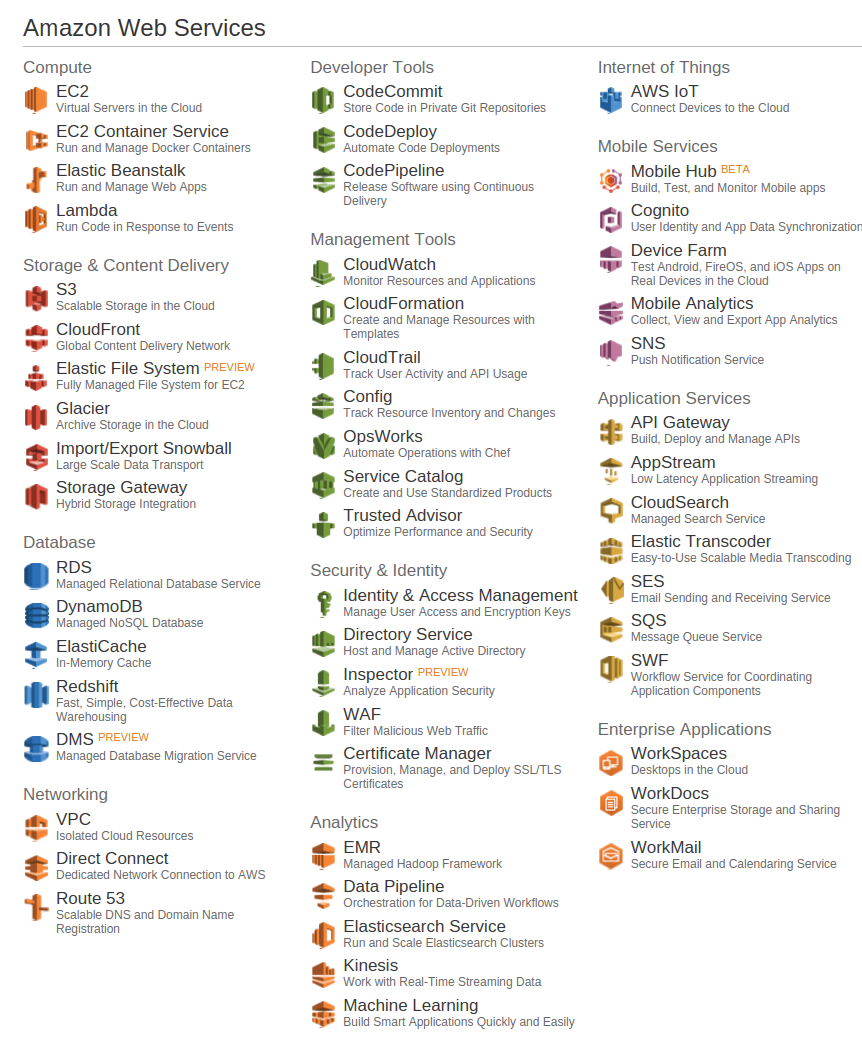
\includegraphics[height=0.8\textheight]{./images/aws-console.png}
		\\
	\end{figure}
\end{frame}


\subsection{Benefits of Moving to Cloud Computing}
\begin{frame}
	\frametitle{\currentname}

	\begin{itemize}
		\item Scalability - built for flexibility
		\item Reduced cost --- services provide the redundancy
		\item No server hardware maintenance
		\item Less maintenance --- more development!
		\item Service provider will have security measures in place
			\begin{itemize}
				\item But is it enough?
			\end{itemize}
		\item Backups can be performed by the service provider --- making sure they are stored correctly
	\end{itemize}

\end{frame}


\subsection{Challenges with Transition to Cloud Computing}
\begin{frame}
	\frametitle{\currentname}

	\begin{itemize}
		\item Privacy concerns
			\begin{itemize}
				\item Under whose jurisdiction?
				\item Are companies happy with having all their customer data offsite?
			\end{itemize}
		\item Support contracts wrt.\ outages
			\begin{itemize}
				\item Especially wrt.\ turnaround
				\item Need to practice redundant DCs
				\item Can the DC's engineers fix it locally? Can the company's engineers fix it remotely?
				\item Every second costs the company money
			\end{itemize}
		\item Is it worth the resource costs?
		\item Not totally in control --- bare metal vs virtualisation
		\item Converting to cloud infrastructure can require restructuring the app
	\end{itemize}
\end{frame}

% http://www.networkworld.com/article/3020235/cloud-computing/and-the-cloud-provider-with-the-best-uptime-in-2015-is.html
% http://www.businessnewsdaily.com/5215-dangers-cloud-computing.html

\begin{frame}[plain]{}
	Questions?
\end{frame}

\end{document}
